\documentclass{article}

\usepackage{float}
\usepackage{caption}
\usepackage{graphicx}
\usepackage{listings}
\usepackage{geometry}
\usepackage[T1]{fontenc}
\usepackage[american]{babel}
\usepackage{csquotes}

\geometry{margin=1in}
\graphicspath{{EEimages/}}

\begin{document}
\author{Chen Xu}
\title{Effectiveness of Various Deep Learning Algorithms on Music Generation}
\maketitle

\section{Introduction}
As technology develops, more and more computationally expensive tasks can be
utilized. One growing field exemplifying this is the category of deep learning
algorithms, that can model very complex data.  Recurrent networks specialize in
this task, being able to model time series, such as speech. This paper will
discuss the effectiveness of using different types of deep learning algorithms
to model another type of time series, music. The model will then be utilized to
generate music, to see how well it is able to model music based on other samples
of music. The model will also be trained using unsupervised learning techniques,
to see the relative abilities of each model to remember sequences, or compress
the music.

\section{Models}
The models that will be used are recurrent neural networks, and other methods
such as restricted boltzmann machines and autoencoders to reduce the
dimensionality of the data before feeding the data into the neural network.

However, in general, all the listed models, have some cost function that they
are trying to minimize. Typically, and in this paper, the cost function is
assumed to be minimized through calculating the gradient of the cost function
with respect to the weights, and then subtracting the gradient from the weights.
This is known as gradient descent.

\subsection{Logistic Regression Model}
To understand learning algorithms, the logistic regression model is notable, as
it is the fundamental building block for larger models. This model predicts a
class based on an input vector of data. Given that: 
$$ \textrm{The input vector} = x$$
and that any value represented by W is a weight matrix that the model learns,
the logistic regression model can be represented as:
$$ \textrm{output} = \sigma(x\cdot W) $$
where:
$$\sigma(x) = \frac{1}{1 + e^{-x}} $$
However, this model typically also includes a bias term, to improve performance,
changing the equation to:
$$ \textrm{output} = \sigma(x\cdot W + b) $$

Logistic regression models typically are used to predict the probability of a
situation or event, based on data. For example, it could be used to predict how
likely someone is to develop cancer based on the data relating to the medical
history of the patient.

\subsection{Neural Networks}
To understand the other models, one must first understand what a neural network
is. Neural networks are a type of model, that attempts to try to learn patterns
within data through stacking logistic regression models on each other. A
logistic regression model predicts a value between 0 and 1 given some data.  To
stack logistic regression classifiers means to put the output of one set of
classifiers as the input as the next set of classifiers. Through this, a neural
network is created.  The neural network was inspired by biological systems, as
the outputs of each classifier can be thought of as activations for synapses in
a brain. These types of models can generally model more complex data than other
models in machine learning literature currently. In practice, however, a neural
network is just a series of matrix operations on an input vector, to calculate
the desired output vector.

\subsection{Deep Learning}
Deep learning simply takes the idea of neural networks, but makes them
significantly larger. Typical neural networks only have 2 through 4 layers,
where each layer is essentially a logistic regression classifier. However,
increasing the number of layers to numbers such as 10 presents considerable
challenges, as it not only takes much longer to compute gradients for the
weights of the network, but the gradients also have a tendency to be too small
or too large, resulting in inefficient training. This problem will be addressed
through using gradient descent algorithms that are not reliant on the magnitude
of the gradient.

Deep learning algorithms however, are capable of much more complex tasks than
neural networks, due to their increased size. Some applications of these deep
networks is SyntaxNet, an algorithm that can correctly determine the grammatical
structure of a sentence, such as determining what the direct object of a
sentence is~\cite{syntaxnet}.


\subsection{Vanilla Recurrent Neural Networks}
Recurrent networks are a variation of neural networks that can model time series
data. This is typically used in speech recognition, as the meaning of a sound in
speech is dependent on the sounds preceding it. Vanilla recurrent neural
networks accomplish this task through being a neural network, except with some
connections going through time.  The activation of a hidden node can be
considered as 
$$a_t = W\cdot a_{t-1} + W\cdot I_t + b_a$$
where $a_t$ is the activation at time t, W is the corresponding weight matrix,
$a_{t-1}$ is the activation of the node at one step before the time, and $I_t$
is the input at that time. The activation typically goes through a nonlinearity,
such as a sigmoid function before being passed to the next node. These models
theoretically can model time series, but in practice they do not have much
memory. As the length of the time series increases, these models become prone to
``forgetting'' earlier samples in the input data. Thus, other more complicated
models should probably be used for time series analysis.

\subsection{Long Short Term Memory Networks}
A model that attempts to overcome the short term memory of vanilla neural
networks is the long short term memory network. These networks, through using
cells and vectors that can be modified by the network, can store long term
information. They do this through generating ``memories'', through the function:
$$M = \tanh(W\cdot C + W\cdot I_t + b_M)$$ where C denotes the cell state of the
network, as originally envisioned by Horchreiter~\cite{lstm}. However, these
networks are significantly more computationally expensive, due to the
significantly increased complexity of the model. As a result, tasks such as
computing the gradient, the error, or predicting something with these models
takes more time than a traditional recurrent neural network.

However, the accuracy of the LSTM can be improved if it is allowed to reset
it's memory state. As originally suggested by Gers, if a LSTM's memory is
multiplied by a ``forget gate'', which is a value between 0 and 1, the LSTM can
predict even longer sequences~\cite{forget}. Through forget gates, the memory of
LSTM's are restrained from growing too large, which would cause the memory cells
to be useless. Also, this addition of a forget gate intuitively, as useless
memory should be discarded. The LSTM's in this paper will be assumed to have
forget gates.

The LSTM accuracy can also be further improved through adding ``peephole
connections''~\cite{lstmpeep}. These are simply a connection between the memory
cell of the LSTM to the forget gates and remember gates. According to Gers'
paper, through these peep hole connections, the LSTM can model short term
changes and fluctuations more accurately.

During training of LSTM's, a notable technique that will be used it large
initialization of the forget gate bias, which if not proper initialized, will
cause problems with the gradient flow of the LSTM~\cite{lstmbias}. Through
initializing a large forget gate, Jozefowicz and others have demonstrated that
this enables LSTM's to learn long term dependencies better, which will also be
used within this paper~\cite{lstmbias}. In this manner, the LSTM mentioned in
this paper will be trained faster.


\subsection{Gated Recurrent Units}
Another variation off of recurrent networks are gated recurrent units, which
follow a similar approach to LSTMs. Instead of completely reassigning the models
hidden state each timestep, it instead updates its hidden state through the
equation:
$$h_t = (1 - z) * h_t + h'_t $$
z is a unit that the model calculates, and is bounded between 0 and 1 with the
sigmoid activation function. As a result, this type of network also has been
found to have long term memories, making it comparable to the performance of
LSTM's. These models also seem to be faster to compute than LSTM's, due to their
lower number of weights. Thus, this model will also be tested against LSTM's in
its performance.


\subsection{Clockwork Recurrent Neural Network}
Another attempt to increase the memory of a vanilla recurrent neural network, is
the clockwork recurrent neural network. Originally developed by Koutnik and his
colleagues, these networks are identical to vanilla networks, except their
hidden layer is partitioned~\cite{cw-rnn}. Each partition of hidden units is
calculated for only some of the input, and thus is not updated at every time
step. As a result, the partitions that are updated less often serve the purpose
of being the memory for the network, and enable the model to ``remember'' better
than normal recurrent networks. Also, these networks are less computationally
expensive than long short term memory networks, resulting in faster compile and
training times. In its original paper, it was concluded that it has
significantly more representational power than LSTM's and GRU's with the same
number of parameters, suggesting that this network is the most efficient network
of them all~\cite{cw-rnn}.

\subsection{Restricted Boltzmann Machines}
The restricted Boltzmann machine is an unsupervised learning algorithm that
attempts to determine the distribution of a sample of input using an energy
based model. This means that the model finds a way to map an ``energy'' to each
input, and then probabilistically finds the lowest energy input. This is useful,
as the model can be trained to associate known input data with lower energy, and
randomly generated data with higher energy. Since this model generates hidden
units to determine the energy of the system, the hidden units can be used as an
input to another model. Typically, the hidden units of a restricted Boltzmann
machine represent some higher level relationship within the data, for example,
the edges of a picture, perhaps. Thus, they can be used to reduce the size of
the input by a significant amount, and speed up the rest of training. Also,
after learning the weights for the restricted boltzmann machine, it is typically
used as a layer for the neural network, which typically speed up training.
However, restricted boltzmann machines are falling out of favor nowadays due to
other initialization techniques for neural networks, and other new activation
functions.

\subsection{Convolution Neural Network}
Convolutional networks are simply an element of a neural network, in which a
filter is applied to all the elements in the input, in some pattern. Typically,
this filter is a n by n matrix, that applied onto an image through multiplying
each pixel value with the corresponding filter value. 
\begin{figure}[H]
	\centering
	\caption{Convolutional Filter}
	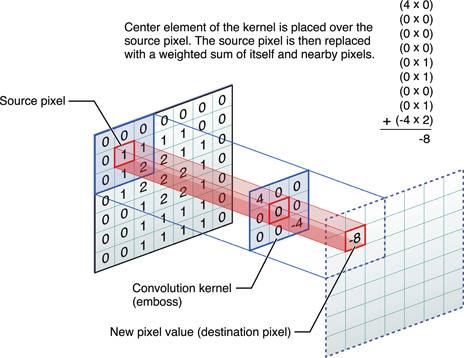
\includegraphics[width=0.8\textwidth]{convolutionFilter.jpg}
\end{figure}
Convolution neural networks are typically used for computer vision technologies,
as elements in an image are generally more related to each other if they are
closer to each other. However, convolutional networks can also be used in time
series analysis, as demonstrated by the research done by
Abdel-Hamid~\cite{convrnn}.


\subsection{Autoencoder}
Autoencoders are also a form of unsupervised learning algorithm, as they simply
find a relationship within the data. They are useful as they can reduce the
dimensionality of the data, making the computations faster for the recurrent
neural network. An autoencoder is a two layer neural network, with the input
layer and desired output both being a sample from the input data. The weights
connecting the input to the hidden layer is generally referred to as the encoder
, and the weights connecting the hidden layer to the output layer is referred to
as the decoder. The hidden layer of the autoencoder is typically passed to more
unsupervised learning algorithms, or the primary model that is to be used.

\begin{figure}[H]
	\centering
	\caption{Simple autoencoder}
	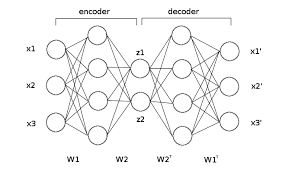
\includegraphics[width=0.7\textwidth]{autoencoderDiagram.jpg}
\end{figure}

The type of autoencoder used in this project will have sigmoid activation
functions, and be trained against mean squared error. The decoder part of the
model will utilize the identity for the activation function, being that no
nonlinearity will be applied to the activations.

\section{Training Techniques}
Because of the aforementioned gradient problems, normal methods of minimizing
the error of these models are extremely slow. Thus, new techniques will be
investigated, although they will not all be tested.

\subsection{Xavier Initialization}
One method to alleviate the vanishing gradient problem is better weight
initialization. As Glorot and Bengio found, the initialization of the weights
affects the propagation of the gradient through the model~\cite{xavier}.
Furthermore, random initialization with a sigmoid activation function causes
problems, as typically the activation value will saturate, due to how the mean
value for a sigmoid function is 0.5. What this means is that since the sigmoid
function has a small gradient around x = 0, once

\subsection{Rprop Trainer}
A training method that was considered was RPROP, originally devised by
Reidmiller and Braun~\cite{rprop}. This training method utilizes only the sign
of the gradient, and has a stored matrix representing the magnitude in which the
algorithm will update the parameters. The reason this method will be used, is
because this algorithm is not affected by the vanishing gradient problem, or the
exploding gradient problem, as the algorithm only worries about the sign of the
gradient, being positive or negative. Furthermore, the algorithm approaches the
minimum for the error function exponentially, as it will increase the magnitude
of the update if the previous update was in the same direction as the current
update. For example, if the first update added 1 to a parameter, and the second
gradient was also positive, the second update would add 1 multiplied with some
constant, being 1.2 in this case. As a result, the updates can potentially
increase exponentially, and will find the gradient with less iterations.
However, this algorithm can only be used for batch learning, and as a result, is
significantly slower for larger datasets. As a result, this training method will
not be used in this paper, although it works for smaller models.

\subsection{RMS Prop}
A technique that was developed by Geoffrey Hinton in one of his lectures, this
technique is a modification to the standard gradient descent method that in
addition, keeps a moving average of the gradients squared~\cite{rmsprop}. Unlike
gradient descent, instead of updating each weight through its gradient, it
divides the calculated gradient by the average square root of the sum of
previous gradients squared. As a result, if a weight constantly receives large
gradients, the update will be divided by a larger value, resulting in the
gradient update not being too large. Similarly, if a gradient for a weight is
extremely small, the gradient will be divided by a smaller average gradient
value, resulting in a larger gradient. Thus, the vanishing and exploding
gradient problem can be resolved through this update mechanism, and furthermore,
this mechanism can be used for mini batch learning as well as batch learning.
Thus, this method is extremely powerful and will be used in the experiments.

\subsection{Back Propagation Through Time}
The gradient for a recurrent neural network differs significantly from a neural
network, in that it is dependent on all the data given to the network before it,
whereas the gradient for a neural network given a data sample, is dependent only
on that data sample. This process of finding the gradient throughout the
previous data samples is known as back propagation through time, as to find the
gradient, one needs to back propagate through the previous data samples, which
are assumed to have occurred earlier in time. Thus, if the data sequence passed
to a recurrent neural network is too long, then training the model will take a
large amount of time.

A modification to this algorithm can be made, to speed up the training, through
learning parts of the data sequence at a time. The hidden variables of the
recurrent model, such as the cell in a long short term memory network can be
generated using the data. Then, instead of calculating the gradient with respect
to all of the data samples, the gradient with respect to only the last, say, 100
data samples can be utilized as an approximation of the gradient, which is
significantly faster. However, as a result, the model will be even less able to
learn long term patterns within the data, due to the gradient not being
calculated with respect to all data samples.


%\subsection{Real Time Recurrent Learning}
%Although back propagation through time is simple to implement, it is
%expensive to calculate, as it requires a complete sequence of data. However,
%another derivation of the derivative of the cost function gives real time
%recurrent learning, which is only dependent on some stored variables, and one
%data sample. However, implementation of this algorithm requires manual
%differention of 

\subsection{Implementational Details}
Python and Theano are used to test these models. Theano is considered to be very
fast amongst the machine learning community, which is why it is used. Also, a
gpu will be utilized to increase the performance of all models. The music
utilized for the model will have come from Youtube. Furthermore, to aid the
model, the music will be put through a Fourier transform before having the model
learn it. This is purely to produce nicer results, as when testing without the
Fourier transform, the model took longer to train and produced more static,
as opposed to the model trained on the Fourier transform.

\section{Comparison}
Thus, this paper will compare the effectiveness of the various models, being
LSTMs, Vanilla Recurrent Networks, and Clockwork Recurrent Neural Networks,
along with different dimensionality reducing steps. The different dimensionality
reducing techniques that will also be tested will be autoencoders, restricted
Boltzmann machines, and convolutional layers.

However, the structure of the models will also be tested. According to the
Google Research Blog, having different overlapping models can help improve
accuracy, so a similar idea will be tested in this paper~\cite{widendeep}.
\section{Data}

\section{Appendix}
As the code is extremely lengthy, it is stored separately. To view the code,
check https://github.com/Peachball/EE-DeepLearning.


\begin{thebibliography}{9}
	\bibitem{deepnetworktrainers}
		Larochelle, Hugo et al. ``Exploring Strategies for Training Deep Neural
		Networks.'' \textit{Journal of Machine Learning Research} (2009): n\. pag.
		Web. 10 May 2016.

	\bibitem{dnn dimensionality}
		Hinton, G.E. and Salakhutdinov, R. R. ``Reducing the Dimensionality of
		Data with Neural Networks.'' \textit{Science} (2006). 504--507. Web. 10
		May 2016

	\bibitem{unsupervised}
		Erhan, Dumitru et al. ``Why Does Unsupervised Pre-training Help Deep
		Learning?'' \textit{University of Montreal}:201--208. Web. 10 May 2016.

	\bibitem{rbm}
		Hinton, Geoffrey. ``A Practical Guide to Training Restricted Boltzmann
		Machines.'' \textit{University of Toronto (2010)}: 1--20. Web. 10 May
		2016.

	\bibitem{rbm intro}
		Fischer, Asja and Igel, Christian. ``An Introduction to Restricted
		Boltzmann Machines. \textit{University of Copenhagen (2012)}: 14--36. Web.
		10 May 2016.

	\bibitem{lstm}
		Horchreiter, Sepp and Schmidhuber, Jurgen. ``Long Short-Term Memory.''
		\textit{Technical University of Munich (1997)}: 1--32. Web. 10 May 2016.

	\bibitem{cw-rnn}
		Koutnik, Jan et al. ``A Clockwork RNN.'' \textit{Dalle Molle Institute
		for Artificial Intelligence Research}: n\. pag. Web. 25 May 2016.

	\bibitem{rmsprop}
		Hinton, Geoffrey. ``Neural Networks for Machine Learning.'' University
		of Toronto. Web. 29 Aug. 2016.

	\bibitem{widendeep}
		Cheng, Heng-Tze. ``Wide and Deep Learning: Better Together with
		Tensorflow.'' \textit{Google Research Blog}, 29 June 2016. Web. 29 Aug.
		2016

	\bibitem{xavier}
		Glorot, Xavier and Bengio, Yoshua. ``Understanding the difficulty of
		training deep feedforward neural networks.'' \textit{Journal of Machine
		Learning Research}, Vol 9, 2010, pag. 249-256. Web. 30 Aug. 2016.

	\bibitem{forgetgate}
		Gers, Schmidhuber, and Cummings. ``Learning to Forget: Continual
		Prediction with LSTM." \textit{ISDIA}, 1999 pag. 1-19. Web. 30 Aug.
		2016.

	\bibitem{syntaxnet}
		Petrov, Slav. ``Announcing SyntaxNet: The World's Most Accurate Parser
		Goes Open Source.'' \textit{Google Research Blob}, 12 May 2016. Web. 20
		Aug. 2016.

	\bibitem{gru}
		Chung, Gulcehre, Cho, and Bengio. ``Empirical Evaluation of Gated
		Recurrent Models on Sequence Modeling.'' \textit{arXiv} Web. 20 Aug.
		2016.

	\bibitem{convrnn}
		Abdel-Hamid, Deng, and Yu. ``Exploring Convolutional Neural Network
		Structures and Optimization Techniques for Speech Recognition.''
		\textit{Microsoft Research}, 2013, pag. 3366-3370. Web. 20 Aug. 2016.

	\bibitem{rprop}
		Riedmiller, Martin and Braun, Henrich. ``A Direct Adaptive Method for
		Faster Backpropagation Learning: The RPROP Algorithm.'' \textit{The
		University of Karlsruhe}, 1993, pag. 586-591. Web. 20 Aug. 2016.

	\bibitem{lstmpeep}
		Gers, Schraudolph, and Schmidhuber. ``Learning Precise Timing with LSTM
		Recurrent Networks.'' \textit{Journal of Machine Learning Research},
		2002, pag. 115-143. Web. 3 Sept. 2016.

	\bibitem{lstmbias}
		Jozefowicz, Zaremba, and Sutskever. ``An Empirical Exploration of Neural
		Network Architectures.'' \textit{JMLR}, vol 37. Web. 4 Sept. 2016.
\end{thebibliography}

\end{document}
